\section{Análisis del problema}

El problema principal que nos concierne es la detección y separación del grano contaminado de la corriente de cereal circulando por los transportadores. Para solucionarlo,
la propuesta de sistema a implementar consiste en la instalación de cámaras infrarojas en la línea de procesado, capaces de captar las imágenes hiperespectrales de la
corriente. De manera que utilizando nuestro modelo previamente calibrado, se detecte cuáles son los granos más contaminados y se puedan separar por una corriente de aire. 
Podemos ver un esquema del sistema en la \textit{imagen\ \ref{fig:detection-system}}.

\begin{figure}
    \centering
    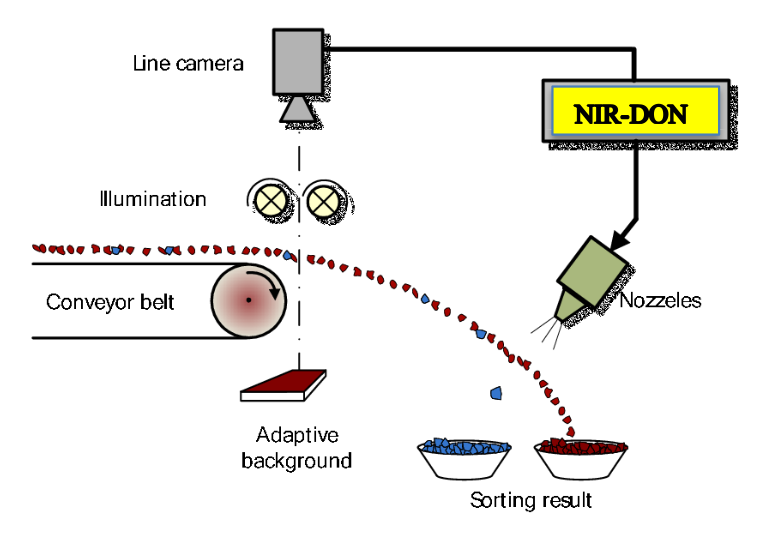
\includegraphics[width=0.7\linewidth]{media/images/esquema-del-sistema.png}
    \caption{Esquema del sistema de detección y filtrado de granos contaminados}\ \label{fig:detection-system}
\end{figure}

Para realizar nuestra parte del proyecto, tenemos una base de datos de imágenes hiperespectrales con formato \acrshort{bil} (\textbf{figura\ \ref{fig:hyperspectral_image}}), 
las cuales simulan las imágenes tomadas en la cadena de producción y de las cuáles hemos extraído los píxeles que forman los granos.
Por otro lado, tenemos una base de datos con el estado de contaminación de estos mismos granos. A partir de ahora utilizaremos los términos contaminación y etiqueta como 
sinónimos a la hora de referirnos a los granos.


\subsection{NIR-HSI}

\gls{nir-hsi} es una tecnología rápida, no destructiva y precisa que nos permite hacer inspecciones de calidad, la cual ha demostrado su potencial en los últimos años\ \cite{Applicat5:online}. 
Es una técnica de imagen química basada en la espectroscopia de reflectancia (la luz reflejada por los materiales), la cual es capaz de caracterizar compuestos orgánicos y 
algunos minerales\ \cite{NIRHyper23:online}.

Como hemos comentado en la introducción, nuestro objetivo es conseguir un modelo que prediga lo mejor posible qué granos de una \gls{imagen hiperespectral} contienen 
granos contaminados con \acrshort{don}. La propuesta general es 


\subsection{Separación del grano contaminado}\ \label{sec:separacion}




El valor de contaminación \gls{don} de un grano lo obtenemos de hacer un proceso químico que no entra dentro del propósito de este proyecto. 
Lo único que nos interesa es que el valor de la contaminación es un valor real. Además, sabemos que desde el laboratorio se considera que un grano está contaminado a 
partir de una concentración de \(1250 \mu g/kg\). De esta forma, aunque es un valor real, podemos utilizarlo como tal o considerar solamente si está contaminado o no. 
Es decir, considerarlo como un problema de \gls{clasificación} o de \gls{regresión}.

Aunque tenemos el valor continuo de contaminación, podemos reemplazarlo directamente por una columna booleana que indique si está contaminado. 
De esta forma pasaríamos de un problema de regresión, el cual nos permite predecir valores continuos, a uno de clasificación para predecir valores discretos, 
si está contaminado o no.

\subsection{Análisis del mercado potencial}





